\documentclass[11pt]{article}

% parameters are fairly self-explanatory here, thankfully
\usepackage[width=7in,height=9.5in,top=0.75in,centering]{geometry}

% for math-ing
\usepackage{amsmath}
\usepackage{amssymb}

\usepackage{tasks}
\newcommand{\tasksA}[2]{\begin{tasks}(#1) #2 \end{tasks}} %use alpha labels

%%%%%% tables %%%%%%%%

\usepackage{array}
\renewcommand{\arraystretch}{1.5}
\setlength{\tabcolsep}{8pt}

%%%%%% plotting %%%%%%

\usepackage[dvipsnames]{xcolor}
\usepackage{tikz}
\usepackage{pgfplots}

\pgfplotsset{every axis/.append style={
                    axis x line=middle,    % put the x axis in the middle
                    axis y line=middle,    % put the y axis in the middle
                    axis line style={<->,color=black}, % arrows on the axis
                    xlabel={$x$},          % default put x on x-axis
                    ylabel={$y$},          % default put y on y-axis
            }}
            
 \pgfplotsset{compat=1.14} % sometimes, everything falls apart without this
 
 %\usepgfplotslibrary{fillbetween} %for shading between curves

%%%%%% commands %%%%%%

% exam heading; course name is first argument, exam information is second argument
\newcommand{\Heading}[2]{
    \fbox{
        {\Large\textbf{#1}}
        }
    \hfill
    \fbox{
        \begin{minipage}{0.2\textwidth}
            \begin{center}
            \textbf{#2}
            \end{center}
        \end{minipage}
    }
    \par\vspace{0.1in}}

% for being lazy while beautifying integrals
\newcommand{\dint}{\displaystyle\int}

% for being lazy while beautifying limits
\newcommand{\dlim}{\displaystyle\lim}

%%%%%% stuff %%%%%%

\usepackage{fancyhdr}

%\setcounter{page}{0} % first page is page 0

\parindent0pt % no indent

\fboxsep=0.25cm % little space in fbox border
%%%%%
%%%% %Jim macros
%%%%%
\newcommand{\sol}[1]{~\\ \col{ {\em Solution: }#1} }
\newcommand{\col}[1]{{\color{blue}#1}} % I frequently use this to indicate where i"m going to be writing something
\newcommand{\al}[1]{\begin{align*} #1 \end{align*}} %\alignment environment without labels
\newcommand{\solbf}[1]{~\\ \col{ {\textbf{Solution: }}#1} }
\newcommand{\tasksI}[2]{\begin{tasks}[style=itemize](#1) #2 \end{tasks}} %use itemize bullets as labels

\def\ds{\displaystyle}
\newcommand{\blue}[1]{{\color{blue}#1}}

\NewDocumentCommand \unlineb { m m g }{% For use in tabular environment
        \IfNoValueTF {#3} {  
            		\underline{ \parbox[c][.25in]{#1in}{\centering \text{\blue{$#2$}}  } } %simulates DJ's \rule[-8pt]{0.75in}{0.4pt}
        }
        {
            		\underline{\parbox[c][#3in][c]{#1in}{\centering \text{\blue{$#2$} } }}
        }
}
\NewDocumentCommand \mpageT { m m o m m }{%First 2 arguments are width of each minipage. Last 2 are contents of each minipage. Optional is to put something in the middle.
        \IfNoValueTF {#3} {  	
        		\begin{minipage}[t]{#1\textwidth}\vspace{0pt}#4 \end{minipage}\begin{minipage}[t]{#2\textwidth}\vspace{0pt}#5 \end{minipage}
        }
        {
		\begin{minipage}[t]{#1\textwidth}\vspace{0pt}#4 \end{minipage} #3 \begin{minipage}[t]{#2\textwidth}\vspace{0pt}#5 \end{minipage}
        }
}
%%%%%
%%%% %Jim macros
%%%%%

%%%%%% BEGIN! %%%%%%%

\begin{document}

\pagestyle{fancy}

% record goals here to create sense of transparency

\fancyhead[c]{%
  \ifcase\value{page}
  % empty test for page = 0
  \or {}% 
  \or {}
  \or
  \or {\bf\color{RedOrange} A2: Local and Absolute Extreme Values}% page=1
  \or {}
  \or {\bf\color{RedOrange} A3: Applied Optimization}% page = 2
  \or {\bf\color{Fuchsia} I1: Meaning of an Integral}% page = 3
  \or {\bf\color{Fuchsia} I2: Properties of Definite Integrals}% page = 4
  \or {\bf\color{Fuchsia} I2: Properties of Definite Integrals}% page = 4
  \or {\bf\color{Fuchsia} I3: Antiderivatives and Indefinite Integrals}% page = 5
  \or {\bf\color{Fuchsia} I4: Compute Definite Integrals}% page = 6
  \or {\bf\color{ProcessBlue} F3: Summations}% page = 7
  \or {\bf\color{Orange} P1: Discrete Random Variables}% page = 8
  \or {\bf\color{Orange} P2: Continuous Random Variables}% page = 9
  \or
  \else
  % Empty chead here!
  \fi
}

\thispagestyle{empty} % don't display that this is page 0

\Heading{MATH 1190/1210 Survey of Calculus I}{Knowledge Checkpoint 4\\Solutions\\Fall 2025}

\vspace{0.1in}

\textbf{Name} \hrulefill \, \begin{minipage}{0.16\textwidth}\begin{center}\textbf{UVA ID\\ (e.g. hdj4nd)} \end{center}\end{minipage}\hrulefill\\

\begin{minipage}{0.2\textwidth}\begin{center}\textbf{Course \&\\ Section Number} \end{center}\end{minipage} \hrulefill\,\,\textbf{Date} \hrulefill  \\

\hrulefill
\paragraph*{Course \& Section Numbers:}

{\small
\begin{center}
\begin{tabular}{| c | c | c | c | c |}
\hline
%
\begin{minipage}{0.12\textwidth}\begin{center}
1190-100\\
J. Rolf\\
(11:00 AM)
\end{center}\end{minipage}
&
\begin{minipage}{0.12\textwidth}\begin{center}
1190-200\\
J. Rolf\\
(9:30 AM)
\end{center}\end{minipage}
&
\begin{minipage}{0.12\textwidth}\begin{center}
1210-100\\
Mikhail\\
(8 AM)
\end{center}\end{minipage}
&
\begin{minipage}{0.12\textwidth}\begin{center}
1210-200\\
Raul\\
(9:30 AM)
\end{center}\end{minipage}
&
\begin{minipage}{0.12\textwidth}\begin{center}
1210-300\\
Sherman\\
(11 AM)
\end{center}\end{minipage}
\\
%
\hline
%
\begin{minipage}{0.12\textwidth}\begin{center}
1210-400\\
Sherman\\
(12:30 PM)
\end{center}\end{minipage}
&
\begin{minipage}{0.12\textwidth}\begin{center}
1210-500\\
Michael\\
(2 PM)
\end{center}\end{minipage}
&
\begin{minipage}{0.12\textwidth}\begin{center}
1210-600\\
J. Bowling\\
(3:30 PM)
\end{center}\end{minipage}
&
\begin{minipage}{0.12\textwidth}\begin{center}
1210-700\\
Josh\\
(9:30 AM)
\end{center}\end{minipage}
&
\begin{minipage}{0.12\textwidth}\begin{center}
1210-800\\
Mason\\
(2 PM)
\end{center}\end{minipage}
\\
%
\hline
%
\begin{minipage}{0.12\textwidth}\begin{center}
1210-900\\
Caelan\\
(3:30 PM)
\end{center}\end{minipage}
&
\begin{minipage}{0.12\textwidth}\begin{center}
1210-920\\
Caelan\\
(5 PM)
\end{center}\end{minipage}
&
\begin{minipage}{0.12\textwidth}\begin{center}
1210-940\\
Mitchell\\
(10 AM)
\end{center}\end{minipage}
&
\begin{minipage}{0.12\textwidth}\begin{center}
1210-950\\
Mitchell\\
(11 AM)
\end{center}\end{minipage}
&
\begin{minipage}{0.12\textwidth}\begin{center}
1210-960\\
Mitchell\\
(noon)
\end{center}\end{minipage}
\\
\hline
\end{tabular}
\end{center}

}

{%\small

\paragraph*{Instructions:}

\begin{itemize}
    
    \item The regular time allowed for completing this assessment is \fbox{$90$} minutes.
    %\item This assessment is out of 50 points.\\
    \item This assessment contains one single-part or multi-part problem for each of the following targets:  {\bf\color{RedOrange}A2}, {\bf\color{RedOrange}A3}, {\bf\color{Fuchsia}I1}, {\bf\color{Fuchsia}I2}, {\bf\color{Fuchsia}I3}, {\bf\color{Fuchsia}I4}, {\bf\color{ProcessBlue}F3}, {\bf\color{Orange}P1}, {\bf\color{Orange}P2}.
    \item On each problem, you will receive a score of Exceeds Expectations (5), Proficient (4), Almost (3), Developing (2), Emerging (1), or Not Yet (0). {\bf Please do not interpret your score as a percentage.}
    %\item You will have opportunities to reassess on the targets appearing on this assessment after the next {\bf 2} assessments.\\
    \item You may NOT use calculators, dictionaries, notes, phones, or any other kind of aid.
    \item Please write neatly. What cannot be read, cannot be graded.
    \item Carefully work out each problem and clearly indicate your final answer to every problem.
    \item Throughout, give the most descriptive answer possible. \textbf{For instance, ``DNE" will not be accepted when ``$=\infty$" is applicable.}
    %\item Please provide the most specific answer possible. For instance, if a limit does not exist because it goes to $\infty$ or $-\infty$, then specify this.
    \item Please use the methods discussed up to this point in the course. For example, any work based on l'H\^opital's Rule will not receive credit.
    \item \textbf{All work must be shown unless otherwise specified.} Partial credit will not be given if appropriate work is not shown.
    \item In particular, {\bf any answer appearing with no justification will receive no credit regardless of whether the answer was correct}, unless otherwise specified.
    \item Please first respond to the prompts on which you feel most proficient, then respond to others later.
    \item This booklet is printed double-sided. It contains 14 pages and 9 numbered problems.
    \item There's a formula sheet on the second-to-last page of common area/volume formulas and optimization concepts in case you need them.
    \end{itemize}
    
    }

\vfill


%%%%%%%%%
\newpage

This page is left blank intentionally.\\

Use this page if you need additional space to write your solutions to any problem. \\

If you wish this page graded, you must refer to this page on \textbf{the original page} of the problem. Otherwise, your grader will NOT consider your work on this page.

\newpage%
%%%%%%%%%


\begin{enumerate}

%%%%%%%%%%%%%%%%%%%%%%%%%%%%%%%%%%%%%%%%%%%%%%%%%%%%%
%%%%%%%%%%% BEGIN PROBLEM A2 %%%%%%%%%%%%%%%%%%%%%%%%
%%%%%%%%%%%%%%%%%%%%%%%%%%%%%%%%%%%%%%%%%%%%%%%%%%%%%

\item Consider the following function $f(x)$ and its derivative.

\[f(x)=3x^5-5x^3\]%-(x-1)^4(15x^2+18x+7)\]

\[f'(x)=15x^2(x-1)(x+1)\]%10(1-x)^3(3x+1)^2\]

You are required to use methods we've learned in our course, such as the first derivative test, the second derivative test, the close interval method, or the first derivative test for absolute extrema, to solve this problem. In addition, you need to make sure the method you use is suitable for the question.

\begin{enumerate}
    \item Find all critical numbers of $f(x)$.

    {\color{blue}\textbf{Solution:}

    If $f'(x)=0$, we get $15x^2(x+1)(x-1)=0$, so $x=-1, 0, 1$.

    There's no $x$-value that makes $f'$ DNE, since $f'$ is a polynomial and is defined for all real numbers.

    $f$ is a polynomial, so all numbers we've found are in its domain. Therefore the critical numbers of $f$ are $x=-1, 0, 1$.

    }

    \item For each critical number found in part (a), classify it as a local minimum, a local maximum, or neither. Fully justify your work.
    
    {\color{blue}\textbf{Solution:}

    $f'(-2)=15(-2)^2(-2-1)(-2+1)=15(4)(-3)(-1)>0$
    
    $f(-0.5)=15(0.5)^2(-0.5-1)(-0.5+1)=15(0.25)(-1.5)(0.5)<0$
    
    $f(0.5)=15(0.5)^2(0.5-1)(0.5+1)=15(0.25)(-0.5)(1.5)<0$
    
    $f(2)=15(2)^2(2-1)(2+1)=15(4)(1)(3)>0$
    
    \begin{center}
    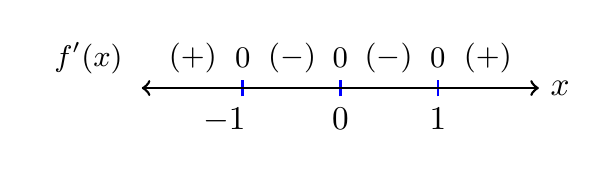
\begin{tikzpicture}[scale=1.2]
                  \begin{axis}[
                  axis y line=left,
                xlabel={$x$},
                ylabel={},
                xlabel style={anchor=west},
    	  y axis line style={draw=none},
    	  	  x axis line style={draw opacity=0},
                %grid = major,
                every major tick/.append style={ thick, blue, major tick length=5pt},
                xtick       = {-1.72, 0, 1.72},
                xticklabels = {$-1\;\;\;\;$ ,$0$,  $1$},
                ytick       = \empty,
                yticklabels={},
                                          y  axis line style=-,
                              % y axis/.append style={y axis line style=-}
                samples     = 320,
                restrict y to domain=-40:40,
                xmin = -5.5, xmax = 3.5,
                ymin = -.5, ymax = 1,
                height=1in, width=2.75in
              ]
    	\draw[thick,<->] (-3.5,0) -- (3.5,0);
    	 \node[anchor=west] at (-5.25,.5) {\small $f^{\prime}(x)$};
    	  \node at (-1.72,.5) {\small $0$};
    	  	   \node at (0,.5) {\small $0$};
    	   \node at (1.72,.5) {\small $0$};
    		\node at (-2.6,.5) {\small $(+)$};
    		\node at (-.85,.5) {\small $(-)$};
    		\node at (.85,.5) {\small $(-)$};
    		\node at (2.6,.5) {\small $(+)$};
              %
            \end{axis}
        \end{tikzpicture}
    \end{center}
    
    By the first derivative test, $f$ has a local maximum at $x=-1$, a local minimum at $x=1$, and neither a local maximum nor a local minimum at $x=0$.}

    {\color{orange} Note: If the second derivative test is used for this part, it cannot be used to classify the critical number x=0. This is because $f''(0)=0$, so the second derivative test is inconclusive. Inconclusive is not neither. It means $x=0$ could be a local max, a local min, or neither, but the test can't come to a conclusion.}

    \item Find the $x$-values of all absolute extrema of $f(x)$ on the interval $[0, 2]$.

    {\color{blue}\textbf{Solution:}
    We look for values of $f(x)$ at all critical numbers in this interval, as well as the endpoints of this interval.
    
    \begin{table}[h!]
        \centering
        \color{blue}
        \begin{tabular}{c|c}
           $x$  & $f(x)$ \\\hline
            $0$ & $0-0=0$\\
            $1$ & $3-5=-2$\\
            $2$ & $3(2)^5-5(2)^3=96-40=56$\\
        \end{tabular}\
    \end{table}
    By comparing these $f(x)$ values, we conclude that on the interval $[0, 2]$, the function $f(x)$ has its absolute maximum value at $x=2$ and has its absolute minimum value at $x=1$.
    }

    {\color{orange} Note: This part is asking for all absolute extrema. The closed interval method is the only suitable method because it is the only method we've learned that would give both absolute max and min. The first derivative test for absolute extrema would only give one absolute extrema, so it would not satisfy what this part is asking for.}
\end{enumerate}

%%%%%%%%%%%%%%%%%%%%%%%%%%%%%%%%%%%%%%%%%%%%%%%%%%%%%%
%%%%%%%%%%%% END PROBLEM A2 %%%%%%%%%%%%%%%%%%%%%%%%%%
%%%%%%%%%%%%%%%%%%%%%%%%%%%%%%%%%%%%%%%%%%%%%%%%%%%%%%

\newpage

%%%%%%%%%%%%%%%%%%%%%%%%%%%%%%%%%%%%%%%%%%%%%%%%%%%%%%
%%%%%%%%%%%% BEGIN PROBLEM A3 %%%%%%%%%%%%%%%%%%%%%%%%
%%%%%%%%%%%%%%%%%%%%%%%%%%%%%%%%%%%%%%%%%%%%%%%%%%%%%%

\item A movie theater has found that if they price movie tickets at \$10 each, they can sell 100 tickets. If the price of each ticket is changed to $p$, then a total number of $n(p)=120-2p$ tickets are sold. There are only 120 seats in the theater.
 
What price should the movie theater sell the tickets at to maximize the revenue?

To receive full credit, make sure to clearly state the objective function, a domain/interval for optimization, and fully justify why price you've found maximizes the revenue. 

You are required to use a method we've learned in our course, such as the first derivative test, the second derivative test, the close interval method, or the first derivative test for absolute extrema, to solve this problem. In addition, you need to make sure the method you use is suitable for the question.

\vspace{.4in}

{\color{blue}\textbf{Solution:} Given the price $p$, the number of tickets sold at that price is $120-2p$, so the revenue function $R(p)$ is $p \cdot (120-2p)$.  (There is a reminder about the meaning/formula for revenue on the formula sheet at the back.)

The number of tickets $120-2p$ cannot be negative, so we must have $p \leq 60$.  Also the price $p$ cannot be negative.  Thus a reasonable domain is $[0,60]$.  It is okay to exclude one or both endpoints, which amounts to requiring that price or attendance be nonzero.

We need to find the \underline{absolute maximum} of the function $R(p) = p \cdot (120-2p) = 120p - 2p^2$ on the domain $[0,60]$.

Let's next find the critical values that lie in the domain, which will be relevant whichever optimization method we choose.  We have $R'(p) = 120 - 4p$, which exists everywhere and is zero when $p=30$.  So the only critical value is 30, which does lie in the domain.

The closed interval method applies, assuming endpoints of the interval were included in the domain.  We compute the revenue at endpoints and critical values in the domain: $R(0)=0$, $R(30) = 1800$, $R(60)=0$.  Thus the maximum revenue is \$1800, attained when the price is \boxed{\$30} per ticket.

OR the first derivative test for absolute extrema applies because there is one critical point in the domain, which is an interval.  One needs to compute the sign of $R'$ on either side of the critical value to get a sign chart, say $R'(10) = 80 > 0$ and $R'(50) = -80 < 0$.  This implies that the critical value of \boxed{\$30} per ticket is an absolute maximum.

}

%%%%%%%%%%%%%%%%%%%%%%%%%%%%%%%%%%%%%%%%%%%%%%%%%%%%%%
%%%%%%%%%%%% END PROBLEM A3 %%%%%%%%%%%%%%%%%%%%%%%%%%
%%%%%%%%%%%%%%%%%%%%%%%%%%%%%%%%%%%%%%%%%%%%%%%%%%%%%%

\newpage

%%%%%%%%%%%%%%%%%%%%%%%%%%%%%%%%%%%%%%%%%%%%%%%%%%%%%%
%%%%%%%%%%%% BEGIN PROBLEM I1 %%%%%%%%%%%%%%%%%%%%%%%%
%%%%%%%%%%%%%%%%%%%%%%%%%%%%%%%%%%%%%%%%%%%%%%%%%%%%%%

\item 

\begin{enumerate}
    \item Let $r(t)$ represent the rate of energy produced by solar radiation per square meter, in kilowatts per square meter, or $kW/m^2$, on a given day, where $t$ is the number of hours since midnight.

    \begin{enumerate}
        \item[(i)] What is the unit of $\displaystyle\int_0^8 r(t)\, dt$?

        {\color{blue}Solution:
        
        $$\frac{\text{kW}}{\text{m}^2} \times \text{hours} = \frac{\text{kW} \times \text{hours}}{\text{m}^2}$$
        }

        \vfill

        \item[(ii)] Explain the meaning of $\displaystyle\int_0^8 r(t)\, dt$ in this context.

        {\color{blue}Solution: The net change in the amount of energy produced between 0 hours and 8 hours since midnight.
    
        OR The total amount of energy produced between 0 hours and 8 hours since midnight.}

        \vfill 
    \end{enumerate}

    \vfill

    \item When bleeding, a human heart still pumps blood, but the amount it pumps drops over time. In particular, the function $p(t)$ represents the amount of blood pumped by the heart per minute, where $t$ represents the number of minutes after the human starts bleeding.

    \begin{enumerate}
        \item[(i)] Based on this scenario, is $\displaystyle \int_0^5 p(t)\, dt$ positive, negative, or 0? No justification required.

        {\color{blue}Solution: Positive, since the heart is still pumping blood, just at a slower rate. Thus, the amount of blood the heart pumped after 5 minutes of bleeding is positive.}

        \vfill

        \item[(ii)] Write down an expression representing the amount of blood the heart pumps from 2 minutes after the start of bleeding to 10 minutes after the start of the bleeding.

        {\color{blue}Solution:
        
        $$\int_2^{10} p(t)dt$$}

        \vfill
    \end{enumerate}

    \vfill
\end{enumerate}


%%%%%%%%%%%%%%%%%%%%%%%%%%%%%%%%%%%%%%%%%%%%%%%%%%%%%%
%%%%%%%%%%%% END PROBLEM I1 %%%%%%%%%%%%%%%%%%%%%%%%%%
%%%%%%%%%%%%%%%%%%%%%%%%%%%%%%%%%%%%%%%%%%%%%%%%%%%%%%

\newpage

%%%%%%%%%%%%%%%%%%%%%%%%%%%%%%%%%%%%%%%%%%%%%%%%%%%%%%
%%%%%%%%%%%% BEGIN PROBLEM I2 %%%%%%%%%%%%%%%%%%%%%%%%
%%%%%%%%%%%%%%%%%%%%%%%%%%%%%%%%%%%%%%%%%%%%%%%%%%%%%%

\item Suppose the following values of definite integrals are given.

\[\int_{-1}^{2}g(x)\,dx=3\]

\[\int_{-3}^{-1}g(x)\,dx=1\]

\[\int_2^{-1}3(f(x)-g(x))\,dx=12\]

\[\int_{-3}^22(f(x)-g(x))\,dx=8\]

Find the value of the following definite integrals.

\tasksA{2}{
\task $\displaystyle\int_2^2 g(x)\, dx$
\textcolor{blue}{
Since an integral over an interval of zero length is always zero, by the \textbf{``Area of a Line Segment Property"}
\\
 $\displaystyle\int_2^2 g(x)\, dx = 0$
}

\task $\displaystyle\int_{-1}^2 f(x)\, dx$
\textcolor{blue}{
We are given:
\[
\int_{-1}^{2} g(x)\,dx = 3,
\qquad
\int_{2}^{-1} 3(f(x)-g(x))\,dx = 12
\]
\textbf{Use ``Reverse Limits Property":}
\[
-\int_{-1}^{2} 3(f(x)-g(x))\,dx = 12
\]
\textbf{Use ``Linearity":}\\
Divide both sides by 3: (algebra)
\[
\int_{-1}^{2} (f(x)-g(x))\,dx = -4
\]
\textbf{Use ``Linearity":}
\[
\int_{-1}^{2} f(x)\,dx - \int_{-1}^{2} g(x)\,dx = -4
\]
Substitute (algebra) \(\int_{-1}^{2} g(x)\,dx = 3\):
\[
\int_{-1}^{2} f(x)\,dx - 3 = -4
\]
\[
\int_{-1}^{2} f(x)\,dx = -1
\]
So, 
\[
\displaystyle\int_{-1}^2 f(x)\, dx = -1
\]
}

\task $\displaystyle\int_{-3}^2 f(x)\, dx$
\textcolor{blue}{
We are given:
\[
\int_{-3}^{2} 2(f(x)-g(x))\,dx = 8
\]
\textbf{Use ``Linearity":}\\
Divide both sides by 2: (algebra)
\[
\int_{-3}^{2} (f(x)-g(x))\,dx = 4
\]
\textbf{Use ``Linearity":}
\[
\int_{-3}^{2} f(x)\,dx - \int_{-3}^{2} g(x)\,dx = 4
\]
\textbf{Use ``Break Apart Property":}\\
Substitute: (algebra)
\[
\int_{-3}^{2} g(x)\,dx
= \int_{-3}^{-1} g(x)\,dx + \int_{-1}^{2} g(x)\,dx
= 1 + 3 = 4
\]
Thus:
\[
\int_{-3}^{2} f(x)\,dx - 4 = 4
\]
\[
\int_{-3}^{2} f(x)\,dx = 8
\]
$\displaystyle\int_{-3}^2 f(x)\, dx = 8$
}}
\textcolor{blue}{
\textbf{Key Aspects of Problem:}
\begin{itemize}
    \item Area of a Line Segment (used once)\\
    \item Reverse Limits Property (used once)\\
    \item Break apart property (used once)\\
    \item Linearity of integration (used four times)\\
    \item Algebraic manipulations (substitution twice and division twice and addition twice)
\end{itemize}
}


%%%%%%%%%%%%%%%%%%%%%%%%%%%%%%%%%%%%%%%%%%%%%%%%%%%%%%
%%%%%%%%%%%% END PROBLEM I2 %%%%%%%%%%%%%%%%%%%%%%%%%%
%%%%%%%%%%%%%%%%%%%%%%%%%%%%%%%%%%%%%%%%%%%%%%%%%%%%%%
%
\newpage

%%%%%%%%%%%%%%%%%%%%%%%%%%%%%%%%%%%%%%%%%%%%%%%%%%%%%
%%%%%%%%%%% BEGIN PROBLEM I3 %%%%%%%%%%%%%%%%%%%%%%%%
%%%%%%%%%%%%%%%%%%%%%%%%%%%%%%%%%%%%%%%%%%%%%%%%%%%%%

\item Assume $x>0$. Write down the indefinite integrals of the following expressions. 

Although no work is required, you are encouraged to include any work that shows your thought process. 

%constant, power, exponential, log, +C, algebraic manipulation

\begin{center}
        \begin{tabular}{l c r l c r}
            %
            $\displaystyle\int x^4+\log_2(10)\,dx$ & $=$ &\unlineb{1.5}{\ds \frac{x^5}{5}+\log_2(10)x+C}{.35} &
            %
            %$\displaystyle\int \,dx$ & $=$ & \rule[-8pt]{1.5in}{0.4pt}\\[0.3in]
            %%%%%
            %$\displaystyle\int 15\,dx$ & $=$ & \rule[-8pt]{1.5in}{0.4pt} & 
            %%%%%
            $\displaystyle\int \dfrac{3}{x^8} \,dx$ & $=$ & \unlineb{1.5}{\ds \frac{3x^{-7}}{-7}+C=-\frac{3}{7x^7}+C}{.35}  \\[.5in]
            %%%%%
            $\displaystyle\int 3^x\,dx$ & $=$ & \unlineb{1.5}{\ds \frac{3^x}{\ln(3)}+C}{.35}&
            %
            $\displaystyle\int \dfrac{1}{2x}\,dx$ & $=$ &  \unlineb{1.5}{\ds \frac{1}{2}\ln|x|+C}{.35} \\[.5in]
            %%%%%
            $\displaystyle\int 4\sqrt{x}-e^x \,dx$ & $=$ &  \unlineb{1.5}{\ds \frac{8}{3}x^{3/2}-e^x+C}{.35} & 
            %
            $\displaystyle\int \dfrac{1}{\sqrt[5]{x^3}} \,dx$ & $=$ &  \unlineb{1.5}{\ds \frac{5}{2}x^{2/5}+C}{.35} \\[0.3in]
            %%%%%
        \end{tabular}
\end{center}

\solbf{
\par\noindent\hrulefill \\
\mpageT{.5}{.5}{
\al{
\int x^4+\log_2(10)\,dx&=\frac{x^5}{5}+\log_2(10)x+C\\
\intertext{($\log_2(10)$ is a constant)}
}
}{
\al{
\int \dfrac{3}{x^8} \,dx&=\int 3x^{-8}\,dx\\
&=3\frac{x^{-7}}{-7}+C\\
&=-\frac{3}{7}\cdot \frac{1}{x^7}+C
}
}
\par\noindent\hrulefill \\
\mpageT{.5}{.5}{
\al{
\int 3^x\,dx&=3^x\cdot\frac{1}{\ln(3)}+C
}
}{
\al{
\int \dfrac{1}{2x}\,dx&=\int \dfrac{1}{2}\cdot \frac{1}{x}\,dx\\
&=\frac{1}{2} \ln|x|+C
}
}
\par\noindent\hrulefill \\
\mpageT{.5}{.5}{
\al{
\int 4\sqrt{x}-e^x \,dx&=\int 4x^{1/2}-e^x \,dx\\
&=4 \cdot \frac{x^{3/2}}{3/2}-e^x +C\\
&=4 \cdot \frac{2}{3}  x^{3/2} - e^x +C\\
&=\frac{8}{3}  x^{3/2} - e^x +C\\
}
}{
\al{
\int \dfrac{1}{\sqrt[5]{x^3}} \,dx&=\int \dfrac{1}{x^{3/5}} \,dx\\
&=\int \dfrac{1}{x^{-3/5}} \,dx\\
&=\frac{x^{2/5}}{2/5}+C\\
&=\frac{5}{2}x^{2/5}+C
}
}
\par\noindent\hrulefill 
}

%%%%%%%%%%%%%%%%%%%%%%%%%%%%%%%%%%%%%%%%%%%%%%%%%%%%%
%%%%%%%%%%% END PROBLEM I3 %%%%%%%%%%%%%%%%%%%%%%%%%%
%%%%%%%%%%%%%%%%%%%%%%%%%%%%%%%%%%%%%%%%%%%%%%%%%%%%%

\newpage

%%%%%%%%%%%%%%%%%%%%%%%%%%%%%%%%%%%%%%%%%%%%%%%%%%%%%%
%%%%%%%%%%%% BEGIN PROBLEM I4 %%%%%%%%%%%%%%%%%%%%%%%%
%%%%%%%%%%%%%%%%%%%%%%%%%%%%%%%%%%%%%%%%%%%%%%%%%%%%%%
%
\item For each of the following definite integrals, determine whether the Fundamental Theorem of Calculus can be applied to evaluate. 

If so, evaluate the integral using the FTC. There's no need to simplify your final answer.

If not, clearly indicate that and explain why.

\begin{enumerate}
    \item $\displaystyle\int_{-8}^{-1}\dfrac{1}{x}+e^x-\sqrt[3]{x}\, dx$\\
\textcolor{blue}{
The integrand is the sum of $\dfrac{1}{x}$, $e^x$, and $-\sqrt[3]{x}=-x^{1/3}$.  On the interval $[-8,-1]$ none of these summands are discontinuous: $1/x$ is defined (zero is not in the interval) and $e^x$ and $-x^{1/3}$ are continuous for all real numbers $x$.  Hence the integrand is continuous on $[-8,-1]$ and the FTC applies.
    The definite integral is then:\\
    \[
    F(x)=\ln|x|+e^x-\frac{3}{4}x^{4/3}\bigg|_{-1}^{-8},
    \]
    since \(\dfrac{d}{dx}\ln|x|=\dfrac{1}{x},\ \dfrac{d}{dx}e^x=e^x,\ \dfrac{d}{dx}\!\left(\frac{3}{4}x^{4/3}\right)=x^{1/3}.\)
    By the FTC,
    \[
    \int_{-8}^{-1}\!\Big(\dfrac{1}{x}+e^x-\sqrt[3]{x}\Big)\,dx
    =F(-1)-F(-8).
    \]
    The evaluated result (left unsimplified) is
    \[
    \boxed{\;\textcolor{blue}{\; \ln|{-1}|+e^{-1}-\tfrac{3}{4}(-1)^{4/3}
    \;-\;\big(\ln|{-8}|+e^{-8}-\tfrac{3}{4}(-8)^{4/3}\big)\;}\;}
    \]
}


    \item $\displaystyle\int_{-8}^1\dfrac{1}{x}+e^x-\sqrt[3]{x}\, dx$\\
    \textcolor{blue}{
     The integrand contains the term $\dfrac{1}{x}$, which is \emph{not} defined at $x=0$.  Because the interval $[-8,1]$ contains $0$, the integrand is not continuous on the entire closed interval $[-8,1]$.  The Fundamental Theorem of Calculus requires the integrand to be continuous on $[a,b]$ in order to apply directly; therefore the FTC \emph{cannot} be applied as stated.\\
    \boxed{\;\textcolor{blue}{\text{FTC cannot be applied because } \dfrac{1}{x}\text{ is undefined at }x=0 \text{ and } 0 \in [-8,1].}\;}}
\end{enumerate}

\textcolor{blue}{
\textbf{Key Aspects of Problem:}
\begin{itemize}
    \item FTC applies to first integral\\
    \item If students conclude that first integral does not satisfy FTC, a domain reason should be given. (Note: the use absolute value in the antiderivative for $\dfrac{1}{x}$ is not being tested on, hence it is not required. So solutions of the form $\ln(-8) - \ln(-1)$ should be counted as valid.)\\
    \item Correct usage of the FTC as the difference in boundary values.\\
    \item Second part does not satisfy FTC\\
    \item Correct reasoning as to why second part does not satisfy FTC. (If students conclude that the second problem does satisfy FTC, a correct implementation should be given with the assumption that it does satisfy the FTC)
\end{itemize}
}

%%%%%%%%%%%%%%%%%%%%%%%%%%%%%%%%%%%%%%%%%%%%%%%%%%%%%%
%%%%%%%%%%%% END PROBLEM I4 %%%%%%%%%%%%%%%%%%%%%%%%%%
%%%%%%%%%%%%%%%%%%%%%%%%%%%%%%%%%%%%%%%%%%%%%%%%%%%%%%
%
%\newpage
%
%%%%%%%%%%%%%%%%%%%%%%%%%%%%%%%%%%%%%%%%%%%%%%%%%%%%%%
%%%%%%%%%%%% BEGIN PROBLEM F3 %%%%%%%%%%%%%%%%%%%%%%%%
%%%%%%%%%%%%%%%%%%%%%%%%%%%%%%%%%%%%%%%%%%%%%%%%%%%%%%

\item 

\begin{enumerate}
    \item Find the value of the following expressions. Simplify as much as possible so that your final answer is a number.

    \begin{enumerate}
        \item[(i)] $\displaystyle\sum_{i=3}^92$

        {\color{blue}\textbf{Solution:}

        $\displaystyle\sum_{i=3}^92=2+2+2+2+2+2+2=14$
    
        }

        \vfill

        \item[(ii)] $\displaystyle\sum_{j=2}^4(j^2-2j)$

        {\color{blue}\textbf{Solution:}

        $\displaystyle\sum_{j=2}^4(j^2-2j)=(2^2-2\cdot 2)+(3^2-2\cdot 3)+(4^2-2\cdot 4)=0+3+8=11$
    
        }

        \vfill
    \end{enumerate}

    \item Write the following sum in summation notation. 

    \[\dfrac{2}{\ln(3)}+\dfrac{4}{\ln(4)}+\dfrac{8}{\ln(5)}+\dfrac{16}{\ln(6)}\]

    {\color{blue}\textbf{Solution:}

    $\displaystyle\sum_{i=3}^6\dfrac{2^{i-2}}{\ln(i)}$ or $\displaystyle\sum_{i=1}^4\dfrac{2^{i}}{\ln(i+2)}$ are two possible correct answers. Other correct answers exist.
    
    }

    \vfill
\end{enumerate}

%%%%%%%%%%%%%%%%%%%%%%%%%%%%%%%%%%%%%%%%%%%%%%%%%%%%%%
%%%%%%%%%%%% END PROBLEM F3 %%%%%%%%%%%%%%%%%%%%%%%%%%
%%%%%%%%%%%%%%%%%%%%%%%%%%%%%%%%%%%%%%%%%%%%%%%%%%%%%%

\newpage

%%%%%%%%%%%%%%%%%%%%%%%%%%%%%%%%%%%%%%%%%%%%%%%%%%%%%%
%%%%%%%%%%%% BEGIN PROBLEM P1 %%%%%%%%%%%%%%%%%%%%%%%%
%%%%%%%%%%%%%%%%%%%%%%%%%%%%%%%%%%%%%%%%%%%%%%%%%%%%%%

\item Let $X$ be a discrete random variable, and let $p(x)$ be its probability mass function.

\begin{enumerate}
    \item Consider the following two tables. It is possible for exactly one of these two tables to be the table for a probability mass function.

    Identify which table can possibly be a probability mass function, fill in the missing value in that table, and use it as the table for $p(x)$. For the one that cannot be a probability mass function, explain why. 

    \vspace{1cm}

    \begin{minipage}{0.45\textwidth}
        \centering    
        \begin{tabular}{c|cccc}
            \hline
           $x$  & 1 & 2 & 3 & 4 \\
           \hline
           $p(x)$  & 0.2 & {\color{blue} 0.35} & 0.15 & 0.3\\
           \hline
        \end{tabular}
    \end{minipage}
    \begin{minipage}{0.45\textwidth}
        \centering
        \begin{tabular}{c|cccc}
            \hline
           $x$  & 1 & 2 & 3 & 4 \\
           \hline
           $p(x)$  & 0.6 &  & 0.35 & 0.2\\
           \hline
        \end{tabular}
    \end{minipage}

    {
      \color{blue}
      We know that for probability mass function $p(x)$ the following has to be true:
      \begin{enumerate}
          \item $p(x) \geq 0$ for any $x$ inside the sample space $S_X$
          \item $\displaystyle\sum_{x \in S_X} p(x) = 1$, i.e. the probabilities have to sum up to 1
      \end{enumerate}
      For the first table, that means:
      $$0.2 + blank+0.15+0.3=1$$
      which means $blank = 1-0.15-0.2-0.3=0.35 \geq 0$
      For the second table,
      $$0.6+0.35+blank+0.2 = 1.15 + blank$$
      There is no way to put a non-negative probability instead of blank to make $1.15+blank=1$, thus this can not be a probability mass function. 
    }
    \vspace{3cm}

    \item Sketch a histogram of the probability mass function $p(x)$.\\
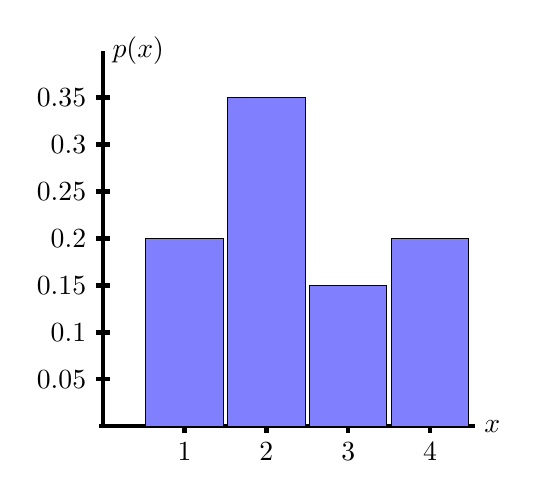
\begin{tikzpicture}
\begin{axis}[
x label style={anchor=west},
xlabel={$x$},
xtick       = {1,2,3,4},
%xticklabels = {$\$0$,$\$40$,$\$80$,$\$120$,$\$160$},
xticklabel style={anchor=north},
y label style={anchor=west},
ylabel={$p(x)$},
ytick       = {0.05, 0.1,0.15, 0.2,0.25,0.30,0.35},
yticklabels = {$0.05$, $0.1$,$0.15$, $0.2$,$0.25$,$0.3$,$0.35$},
enlarge x limits={.01}, % Adjusts spacing between bars and axis limits
samples     = 320,
xmin =0, xmax = 4.5,
ymin = 0, ymax = .4,
axis line style = { ultra thick, -},
every major tick/.append style={ultra thick, black, major tick length=5pt},
width=2.5in, height=2.5in
]
\addplot[ybar, bar shift=0,   bar width=28pt,  fill=blue!50] plot coordinates { (1,0.2)  (2,0.35) (3,0.15) (4,0.2) };
\end{axis}
\end{tikzpicture}
%


    \item Find $P(X\text{ is even})$.
    
    {
    \color{blue}
    $P(X\text{ is even}) = P(X=2) + P(X=4) = p(2) + p(4) = 0.35+0.3=0.65$
    }
    \vfill

\end{enumerate}

%%%%%%%%%%%%%%%%%%%%%%%%%%%%%%%%%%%%%%%%%%%%%%%%%%%%%%
%%%%%%%%%%%% END PROBLEM P1 %%%%%%%%%%%%%%%%%%%%%%%%%%
%%%%%%%%%%%%%%%%%%%%%%%%%%%%%%%%%%%%%%%%%%%%%%%%%%%%%%

\newpage

%%%%%%%%%%%%%%%%%%%%%%%%%%%%%%%%%%%%%%%%%%%%%%%%%%%%%%
%%%%%%%%%%%% BEGIN PROBLEM P2 %%%%%%%%%%%%%%%%%%%%%%%%
%%%%%%%%%%%%%%%%%%%%%%%%%%%%%%%%%%%%%%%%%%%%%%%%%%%%%%
%
\item Let $X$ represent the number of day a light bulb lasts. Suppose the light bulb lasts at most 100 days.

\begin{center}
    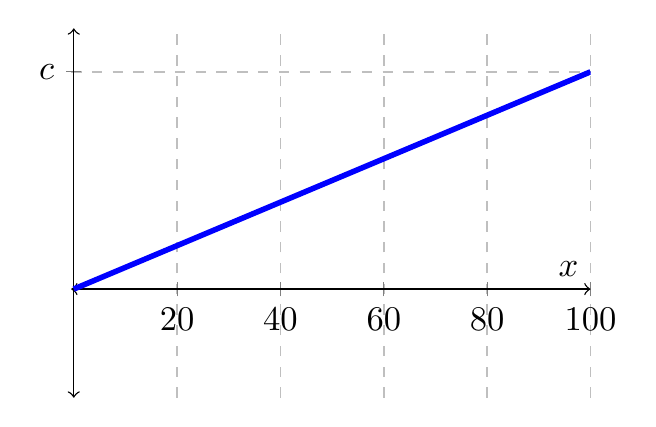
\begin{tikzpicture}[scale=1.25]
          \begin{axis}[
            xlabel={$x$},
            ylabel={\empty},
            %grid = major,
            xtick       = {0,20,40,60,80,100},
            xticklabels = {$0$,$20$,$40$,$60$,$80$,$100$},
            ytick       = {0,1},
            yticklabels = {$0$, $c$},
            samples     = 320,
            domain      = 0:101,
            restrict y to domain=-2:5,
            xmin = -0.5, xmax = 100,
            ymin = -0.5, ymax = 1.2,
            height=2.1in, width=2.7in,
            grid=both, grid style=dashed]
            %\addplot[domain=0:4, blue, ultra thick, mark=none] {4-4/2^x};
            %\addplot[domain=5:8, blue, ultra thick, mark=none] {};
            %\node at (4,3) {$r(t)$};
            \draw[ultra thick, blue] (0,0) -- (100, 1);
        \end{axis}
        
    \end{tikzpicture}
    \end{center}

\begin{enumerate}
    \item The graph above is the cumulative distribution function of $X$. What should the value of $C$ be?

    {\color{blue} Solution: $C = 1$ because $C(x) = 1$ at the upper end of the support (in this case, at $x = 100$).}

    \vfill

    \item Find the formula of the probability density function $p(x)$ of $X$.

    {\color{blue} Solution: Since $C = 1$, then we can calculate the line above to have the equation for the cumulative density function:
    
    $$C(x) = \begin{cases}
        0 &\text{ if } x < 0 \\
        \frac{x}{100} &\text{ if } 0 \leq x \leq 100 \\
        1 &\text{ if } x > 1
    \end{cases}$$
    
    Since we know the probability density function is the derivative of the cumulative function, then

    $$p(x) = C'(x) = \begin{cases}
        \frac{1}{100} &\text{ if } 0 \leq x \leq 100 \\
        1 &\text{ otherwise}
    \end{cases}$$}

    \vfill

    \item What is the probability that the light bulb lasts less than 60 days?

    {\color{blue} We can use the probability density function:
    
    $$P(X \leq 60) = \int_0^{60} p(x) dx = \int_0^{60} \frac{1}{100} dx = \frac{x}{100} \bigg|_0^{60} = \frac{60}{100} - \frac{0}{100} = 0.6 = 60\%$$
    
    OR we can use the cumulative density function:
    
    $$P(X \leq 60) = C(60) = \frac{60}{100} = 0.6 = 60\%$$}

    \vfill
\end{enumerate}



%%%%%%%%%%%%%%%%%%%%%%%%%%%%%%%%%%%%%%%%%%%%%%%%%%%%%%
%%%%%%%%%%%% END PROBLEM P2 %%%%%%%%%%%%%%%%%%%%%%%%%%
%%%%%%%%%%%%%%%%%%%%%%%%%%%%%%%%%%%%%%%%%%%%%%%%%%%%%%

\newpage

\begin{center}
{\bf DO NOT REMOVE THIS SHEET FROM YOUR EXAM PACKET}
\end{center}

\begin{center}
    \begin{tabular}{ r | c | l }
    {\bf Description} & {\bf Formula} & {\bf Variables}\\
    \hline
    area of a square & $A=s^2$ & $s=$ side length\\
    \hline
    area of a rectangle & $A=lw$ & $l=$ length, $w=$ width\\
    \hline
    area of a triangle & $A=\frac12bh$ & $b=$ base, $h=$ height\\
    \hline
    area of a circle & $A=\pi r^2$ & $r=$ radius\\
    \hline
    volume of a rectangular box & $V=lwh$ & $l=$ length, $w=$ width, $h=$ height\\
    \hline
    %volume of a circular cylinder & $V=\pi r^2 h$ & $r=$ radius, $h=$ height\\
    %\hline
    %volume of a sphere & $V=\frac43\pi r^3$ & $r=$ radius\\
    %\hline
    revenue & $R(x) = p\cdot x = p\cdot Q$ & $p=$ unit price, $x=Q=$ quantity sold\\
    \hline
    profit & $P(x) = R(x) - C(x)$ & $R(x)=$ revenue, $C(x)=$ cost\\
    \hline
    average cost & $\overline C(x) = \frac{C(x)}{x}$ & $C(x)=$ cost\\
    \end{tabular}
\end{center}

\begin{center}
{\bf DO NOT REMOVE THIS SHEET FROM YOUR EXAM PACKET}
\end{center}

\newpage

This page is left blank intentionally.\\

Use this page if you need additional space to write your solutions to any problem. \\

If you wish this page graded, you must refer to this page on \textbf{the original page} of the problem. Otherwise, your grader will NOT consider your work on this page.

\newpage

This page is left blank intentionally.\\

Use this page if you need additional space to write your solutions to any problem. \\

If you wish this page graded, you must refer to this page on \textbf{the original page} of the problem. Otherwise, your grader will NOT consider your work on this page.


\end{enumerate}

\end{document}